\begin{figure}[htbp]
\centering
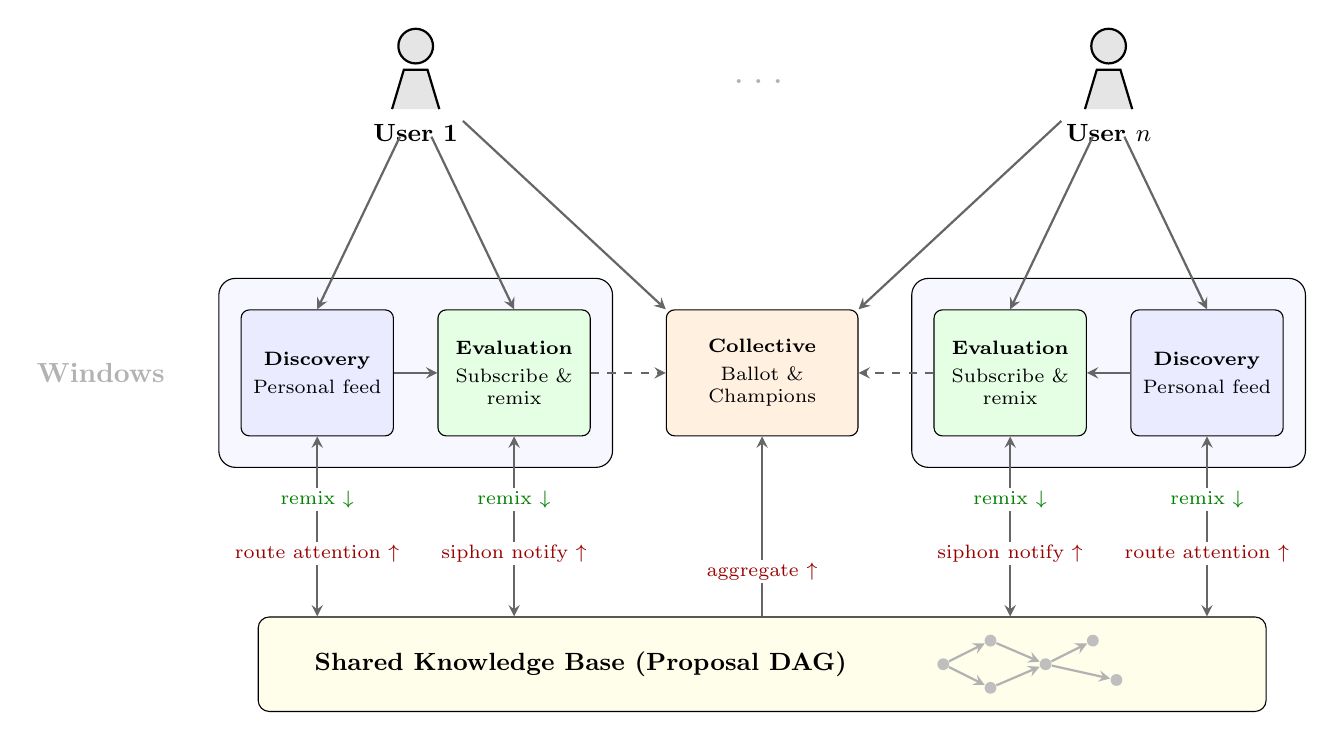
\begin{tikzpicture}[
    >=stealth,
    % Styles
    window/.style={draw, rounded corners=3pt, fill=#1, 
        minimum width=1.8cm, minimum height=1.6cm, font=\scriptsize,
        align=center, text width=1.7cm},
    dagbox/.style={draw, rounded corners=4pt, fill=yellow!8, 
        minimum width=12.8cm, minimum height=1.2cm},
    planelabel/.style={font=\scriptsize\scshape, text=gray!70},
    leveltext/.style={font=\scshape\bfseries, text=gray!60, align=right}
]

% --- Users ---
\node (user1) at (-4.4, 0) {};
\node (userN) at (4.4, 0) {};
\node[font=\LARGE, text=gray!60] at (0, -0.3) {\dots};

% User 1 icon
\draw[thick, fill=gray!20] (-4.4, 0.15) circle (0.22);
\draw[thick, fill=gray!20] (-4.7, -0.65) -- (-4.55, -0.15) -- (-4.25, -0.15) -- (-4.1, -0.65);
\node[font=\small\bfseries, below=0.02cm] at (-4.4, -0.7) {User 1};

% User N icon
\draw[thick, fill=gray!20] (4.4, 0.15) circle (0.22);
\draw[thick, fill=gray!20] (4.1, -0.65) -- (4.25, -0.15) -- (4.55, -0.15) -- (4.7, -0.65);
\node[font=\small\bfseries, below=0.02cm] at (4.4, -0.7) {User $n$};

% --- Level Labels ---
\node[leveltext] at (-8.4, -4.0) {Windows};

% --- Window planes ---
\node[draw, rounded corners=6pt, fill=blue!3, minimum width=5.0cm, minimum height=2.4cm] (box1) at (-4.4, -4.0) {};
\node[draw, rounded corners=6pt, fill=blue!3, minimum width=5.0cm, minimum height=2.4cm] (boxN) at (4.4, -4.0) {};

% --- Windows ---
\node[window=blue!8] (disc1) at (-5.65, -4.0) {\textbf{Discovery}\\[2pt]Personal feed};
\node[window=green!10] (eval1) at (-3.15, -4.0) {\textbf{Evaluation}\\[2pt]Subscribe \&\\remix};

\node[window=green!10] (evalN) at (3.15, -4.0) {\textbf{Evaluation}\\[2pt]Subscribe \&\\remix};
\node[window=blue!8] (discN) at (5.65, -4.0) {\textbf{Discovery}\\[2pt]Personal feed};

\node[window=orange!12, minimum width=2.4cm, text width=2.2cm] (collective) at (0, -4.0) {\textbf{Collective}\\[2pt]Ballot \& Champions};

% --- Arrows from Users to Windows ---
% User 1
\draw[->, thick, gray!80!black] (-4.6, -1.0) -- (disc1.north);
\draw[->, thick, gray!80!black] (-4.2, -1.0) -- (eval1.north);
\draw[->, thick, gray!80!black] (-3.8, -0.8) -- (collective.north west);
% User N
\draw[->, thick, gray!80!black] (4.6, -1.0) -- (discN.north);
\draw[->, thick, gray!80!black] (4.2, -1.0) -- (evalN.north);
\draw[->, thick, gray!80!black] (3.8, -0.8) -- (collective.north east);

% --- Horizontal Influence Arrows ---
\draw[->, thick, gray!80!black] (disc1.east) -- (eval1.west);
\draw[->, thick, gray!80!black, dashed] (eval1.east) -- (collective.west);
\draw[->, thick, gray!80!black] (discN.west) -- (evalN.east);
\draw[->, thick, gray!80!black, dashed] (evalN.west) -- (collective.east);

% --- DAG ---
\node[dagbox] (dag) at (0, -7.7) {};
\node[anchor=east, font=\small\bfseries] at (1.2, -7.7) {Shared Knowledge Base (Proposal DAG)};

% DAG Icon next to text
\begin{scope}[every node/.style={circle, fill=gray!50, minimum size=0.15cm, inner sep=0pt}]
    \node (n1) at (2.3, -7.7) {};
    \node (n2) at (2.9, -7.4) {};
    \node (n3) at (2.9, -8.0) {};
    \node (n4) at (3.6, -7.7) {};
    \node (n5) at (4.2, -7.4) {};
    \node (n6) at (4.5, -7.9) {};
\end{scope}
\begin{scope}[->, thick, gray!60]
    \draw (n1) -- (n2);
    \draw (n1) -- (n3);
    \draw (n2) -- (n4);
    \draw (n3) -- (n4);
    \draw (n4) -- (n5);
    \draw (n4) -- (n6);
\end{scope}

% --- Window <-> DAG connections ---
\draw[<->, thick, gray!80!black] (disc1.south) -- (disc1.south |- dag.north)
    node[pos=0.35, fill=white, inner sep=1pt, font=\scriptsize, text=green!50!black] {remix $\downarrow$}
    node[pos=0.65, fill=white, inner sep=1pt, font=\scriptsize, text=red!60!black] {route attention $\uparrow$};
\draw[<->, thick, gray!80!black] (discN.south) -- (discN.south |- dag.north)
    node[pos=0.35, fill=white, inner sep=1pt, font=\scriptsize, text=green!50!black] {remix $\downarrow$}
    node[pos=0.65, fill=white, inner sep=1pt, font=\scriptsize, text=red!60!black] {route attention $\uparrow$};
\draw[<-, thick, gray!80!black] (collective.south) -- (collective.south |- dag.north)
    node[pos=0.75, fill=white, inner sep=1pt, font=\scriptsize, text=red!60!black] {aggregate $\uparrow$};

% Eval1 <-> DAG (Siphon left)
\draw[<->, thick, gray!80!black] (eval1.south) -- (eval1.south |- dag.north) 
    node[pos=0.35, fill=white, inner sep=1pt, font=\scriptsize, text=green!50!black] {remix $\downarrow$}
    node[pos=0.65, fill=white, inner sep=1pt, font=\scriptsize, text=red!60!black] {siphon notify $\uparrow$ };

% EvalN <-> DAG (Siphon right)
\draw[<->, thick, gray!80!black] (evalN.south) -- (evalN.south |- dag.north) 
    node[pos=0.35, fill=white, inner sep=1pt, font=\scriptsize, text=green!50!black] {remix $\downarrow$}
    node[pos=0.65, fill=white, inner sep=1pt, font=\scriptsize, text=red!60!black] {siphon notify $\uparrow$};

\end{tikzpicture}
\caption{System architecture overview. Multiple users interact with the shared knowledge base through individual \textit{Discovery} and \textit{Evaluation} windows, while observing a shared \textit{Collective Window}. The individual windows feed sequentially into the collective view, driven by user evaluations, which in turn feeds back into the Discovery windows. The Siphon Effect creates a feedback loop: new remixes in the DAG trigger notifications to existing subscribers via their Evaluation window.}
\label{fig:system-architecture}
\end{figure}
